\begin{figure*}[t]
\centering
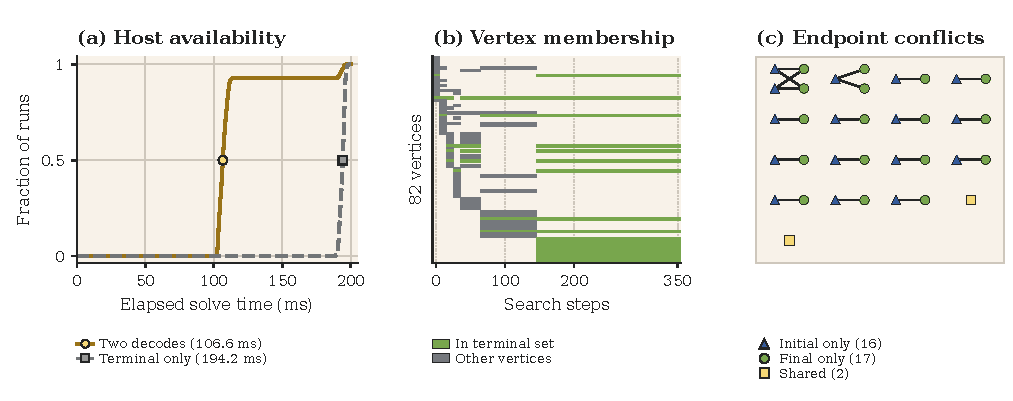
\includegraphics[width=\textwidth]{figures/decode_cases.pdf}
\caption{\textbf{Host availability and changing membership in SPRINT-S.} (a) Across 3,000 small RB graph--seed pairs, the median time at which the ultimately scored set reaches the host is 106.6~ms with two decodes and 194.2~ms with terminal-only decoding. Markers locate the medians on the cumulative curves. (b) A separate fixed-work run on the first RB graph (242 vertices, 2,393 edges, seed 1017) decodes the top four archive entries every ten steps. Each row tracks one vertex. Filled cells mark membership at that checkpoint, and green identifies vertices that belong to the terminal set. Size reaches 19 at step ten and stays there while membership changes. (c) The union of the initial and final sets induces 19 conflict edges. The two shared vertices are isolated.}
\label{fig:decode-cases}
\end{figure*}
